\documentclass[12pt]{article}
\usepackage[a4paper, total={6in, 9in}]{geometry}
\usepackage{graphicx}
\graphicspath{ {./images/output/} }
\usepackage{caption}
\usepackage[english]{babel}
\usepackage{titling}
\usepackage{float}
% \usepackage{amsmath}
% \usepackage{minted}
% \usepackage{multicol}
% \usepackage{array}
% \usepackage{setspace}
% \usepackage{placeins}

% \usepackage{lipsum}

\title{Full Wave Bridge Rectifier Using Diodes}
\author{}
\date{}

\pagenumbering{gobble}
\begin{document}

\pagebreak
\pagenumbering{arabic}
\maketitle

\section*{Objective}
\addcontentsline{toc}{section}{Objective}
\begin{itemize}
    \item To construct a single-phase full-wave bridge rectifier using diodes.
    \item To analyze the output waveforms for resistive and inductive loads.
    \item To understand the working principle of a full-wave bridge rectifier.
\end{itemize}

\section*{Circuit Diagrams}
\addcontentsline{toc}{section}{Circuit Diagrams}
\begin{figure}[H]
    \centering
    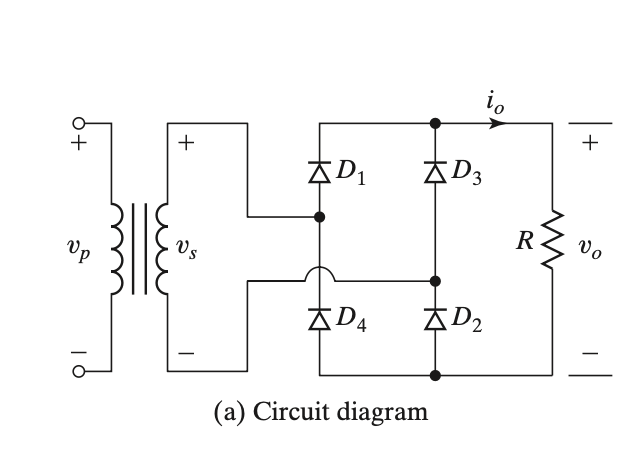
\includegraphics[width=.5\textwidth]{bridge_ckt.png}
    \caption{Full Wave Bridge Rectifier Circuit \cite{rashid2013power}}
    \label{fig:dc_r_load}
\end{figure}

\section*{Observations}
\addcontentsline{toc}{section}{Observations}
\begin{itemize}
    \item Constructed a full-wave bridge rectifier using four diodes.
    \item Observed output waveforms for resistive and inductive loads.
    \item Verified continuous conduction through the bridge for both half-cycles.
    \item Confirmed that the output DC voltage is smoother compared to a half-wave rectifier.
\end{itemize}

\subsubsection*{Outputs}
\begin{figure}[H]
    \centering
    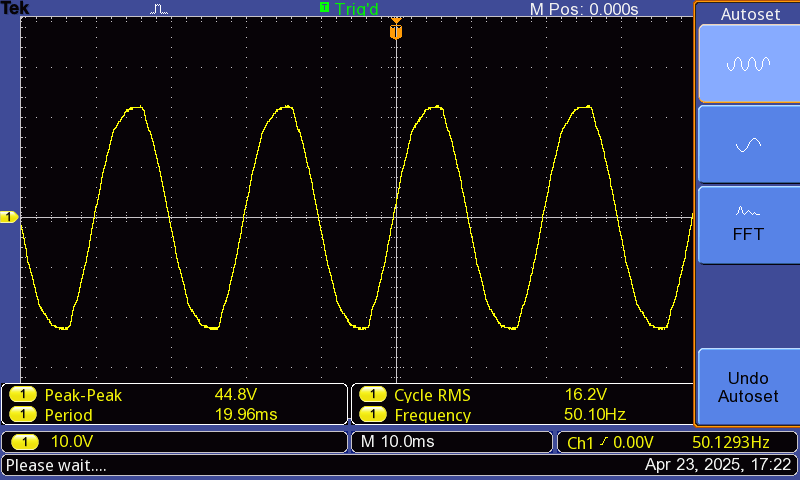
\includegraphics[width=.8\textwidth]{fullb_r_load6_in.png}
    \caption{Full wave rectifier input voltage signal}
    \label{fig:rLoad}
\end{figure}

\begin{figure}[H]
    \centering
    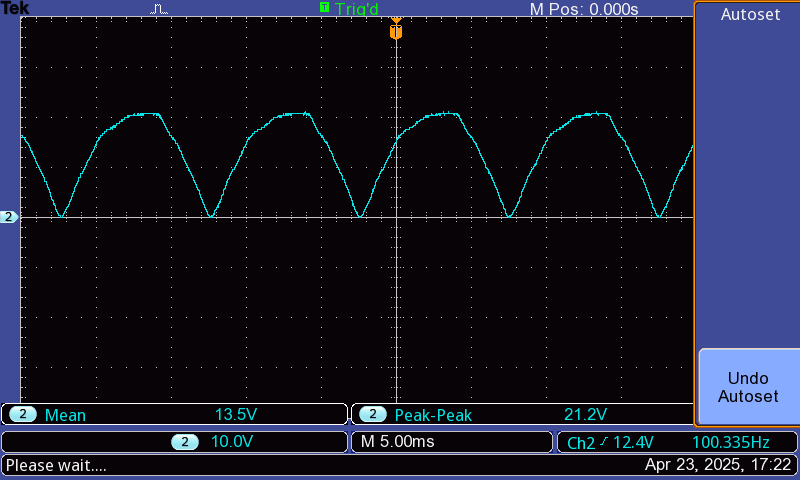
\includegraphics[width=.8\textwidth]{fullb_r_load6_out.png}
    \caption{Full wave rectifier output voltage signal}
    \label{fig:rLoadDelay}
\end{figure}

\bibliographystyle{IEEEtran}
\renewcommand{\bibname}{References}
\addcontentsline{toc}{section}{References}
\bibliography{ref}


\end{document}
